\documentclass{article}
\usepackage{fullpage}
\usepackage{graphicx}

\title{16.35 PSet \#2}
\author{Ryan Fish}
\date{\today}

\begin{document}
\maketitle

\section{VehicleController}
\section{GroundVehicle}
\subsection{Requirements}
\subsubsection{Variables}
\begin{enumerate}
	\item \verb|pose[]| shall be an array of exactly 3 elements that determine the position and orientation of a vehicle on a 2D plane.
	\begin{enumerate}
		\item \verb|pose[0]|, which represents the x-coordinate of said vehicle, shall remain at all times within the range $[0,100]$.
		\item \verb|pose[1]|, which represents the y-coordinate of said vehicle, shall remain at all times within the range $[0,100]$.
		\item \verb|pose[2]|, which represents the yaw of said vehicle, shall remain at all times within the range $[-\pi, \pi)$.
		\begin{enumerate}
			\item If the vehicle would otherwise be set to a value outside of these bounds, the value shall be wrapped to the equivalent angle within the range.
		\end{enumerate}
	\end{enumerate}
	\item \verb|speeds[]| shall be an array of exactly 2 elements that determine the derivative of position and orientation.
	\begin{enumerate}
		\item \verb|speeds[0]|, which represents the absolute linear velocity of said vehicle, shall remain at all times within the range $[3,10]$.
		\begin{enumerate}
			\item In order to maintain a no-slip condition, the linear velocity shall be described only as a magnitude, with the variable described by \verb|1(c)| determining the direction of motion.
		\end{enumerate}
		\item \verb|speeds[1]|, which represents the rotational velocity of said vehicle, shall remain at all times within the range $[-\pi/4,\pi/4]$ .
	\end{enumerate}
\end{enumerate}
\subsubsection{Construction}
\begin{enumerate}
	\item There shall be one constructor for the \verb|GroundVehicle| object.  The constructor shall take 3 inputs.
	\begin{enumerate}
		\item The first input shall be an array defining the vehicle starting position as defined in 2.1.1.1
		\item The second input shall be a value defining the vehicle linear velocity as defined in 2.1.1.2(a)
		\item The third input shall be a value defining the vehicle rotational velocity as defined in 2.1.1.2(b)
	\end{enumerate}
	\item If any inputs are invalid in range as described by 2.1.1.1 and 2.1.1.2, but valid in type, the constructor shall set the inputs to their nearest legal bounds and result in a valid object being returned.
	\item If the inputs to the constructor are invalid in number or type, the constructor shall throw an error signifying invalid inputs.
\end{enumerate}
\subsubsection{Methods}
\begin{enumerate}
	\item \verb|getPosition|
	\begin{enumerate}
		\item The method shall take nothing as input.
		\item The method shall return, as an array, the vehicle position as defined in 2.1.1.1
	\end{enumerate}
	\item \verb|getVelocity|
	\begin{enumerate}
		\item The method shall take nothing as input.
		\item The method shall return, as an array with three values, the vehicle velocities.
		\begin{enumerate}
			\item The first element of the returned array shall be the x component of the vehicle's velocity in the coordinate frame from which the vehicle orientation is referenced.
			\item The second element of the returned array shall be the y component of the vehicle's velocity in the coordinate frame from which the vehicle orientation is referenced.
			\item The third element of the returned array shall be the rotational component of the vehicle's velocity.
		\end{enumerate}
	\end{enumerate}
	\item \verb|setPosition|
	\begin{enumerate}
		\item The method shall take as input an array as defined in 2.1.1.1
		\item The method shall validate the inputs in a manner consistent with 2.1.2.2 and 2.1.2.3
		\item The method shall set the vehicle \verb|pose[]| variable to the input array.
	\end{enumerate}
	\item \verb|setVelocity|
	\begin{enumerate}
		\item The method shall take as input an array as defined in 2.1.3.2(b)
		\item The method shall validate the inputs in a manner consistent with 2.1.2.2 and 2.1.2.3
		\item The method shall set the linear velocity as defined in 2.1.1.2(a) as the euclidean norm of the first two input array elements.
		\begin{enumerate}
			\item To ensure consistency of the no-slip condition, the method shall also set the vehicle heading as defined in 2.1.1.1(c) to that of the vector resultant of the sums of the input x and y velocities.
		\end{enumerate}
		\item The method shall set the rotational velocity as defined in 2.1.1.2(b) to the value of the third array element.
	\end{enumerate}
	\item \verb|controlVehicle|
	\begin{enumerate}
		\item The method shall take as input a single instance of a \verb|Control| object.
		\item The method shall validate the input in a manner consistent with 2.1.2.3
		\item The method shall return immediately upon receiving a null \verb|Control| object.
		\item The method shall validate the velocity fields of the \verb|Control| object in a manner consistent with 2.1.1.2
		\item The method shall set the linear and rotational velocity fields as defined in 2.1.1.2 of the vehicle to the values stored in the respective fields of the \verb|Control| object.
	\end{enumerate}
	\item \verb|updateState|
	\begin{enumerate}
		\item The method shall take as input two arguments
		\begin{enumerate}
			\item An unsigned integer representing the time since the vehicle started in seconds, floored.
			\item An unsigned integer representing the additional microseconds elapsed since the time given in the first argument.
			\item If both inputs are 0, the method shall preemptively exit.
			\item If either input is signed, the method shall exit, throwing an error signifying invalid inputs.
		\end{enumerate}
		\item The method shall validate the input in a manner consistent with 2.1.2.3
		\item The method shall set the new position of the vehicle based on the time elapsed and the vehicle speeds as of the update.
		\begin{enumerate}
			\item The final position shall not exceed the limits stated in 2.1.1.1
			\item The delta between the current and final position shall be approximated as a straight line in the case that the absolute value of the rotational velocity as defined in 2.1.1.2b is less than $s*2*\pi*MIN\_VALUE$, where \verb|MIN_VALUE| is defined as the value closest to 0 of the data primitive used.
			\item If the absolute value of the rotational velocity exceeds that specified in 2.1.3.6(c)ii, the exact, partial-arc solution shall be used in calculating the new position.  The $2*\pi$ divided by the rotational velocity determines the time the vehicle would take to rotate through a full circle.  This time multiplied by the linear velocity determines the circumference of that circle, and therefore its radius and diameter.  The new position of the vehicle is given by the arc segment given by the update duration times the rotational velocity, of the circle tangent to the vehicle's current vehicle with the radius previously calculated.
		\end{enumerate}
	\end{enumerate}
\end{enumerate}
\subsection{Unit Tests}
I have not included unit tests for some of the Ground Vehicle functionality due to it having been tested in the previous assignment.  New functionality is being tested as part of the behavior of the other classes.
\section{Simulator}
\subsection{Normal Polygon Sim}
\begin{figure}
\centering
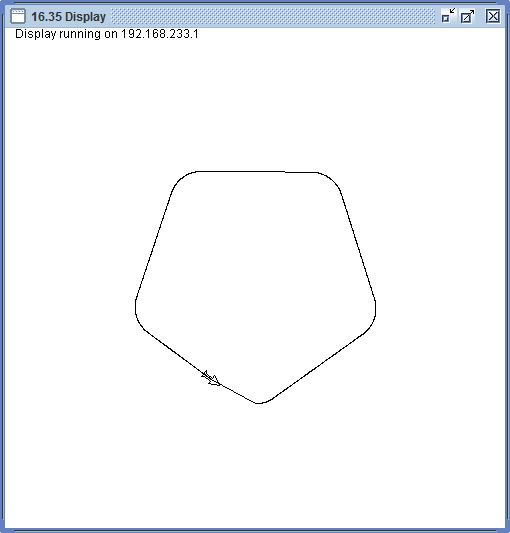
\includegraphics[width=0.7\linewidth]{pentagon}
\caption{pentagon}
\label{fig:pentagon}
\end{figure}


\section{Mutex and Sync}
\subsection{Shared Resources}
\begin{enumerate}
	\item Each \verb|GroundVehicle| is shared between threads
	\item The time is controlled from \verb|Simulator|, but read from many.
	\item The \verb|GroundVehicle| position is controlled from one thread, but read from many.
	\item The status variable indicating all \verb|VehicleControllers| have completed needs to be read and written by many.
\end{enumerate}
\subsection{Critical Regions}
\begin{enumerate}
	\item Modifying the state of the \verb|GroundVehicle|, as in, changing velocity or position, should be done from one and only one thread at a time.
	\item Modifying time must be a mutex operation, so listening threads never read a partially updated variable.
	\item The position output to the client is managed by one thread, but many threads have updated positions.  Changing the pose of a vehicle must be done in mutex, and the output to the client shall be managed by a single thread, using a buffer that has atomic write operations.
	\item Incrementing the status variable to indicate thread cycle completion shall be a mutex operation, as well as locking, to protect from READ-READ-MODIFY-WRITE-MODIFY-WRITE style errors.
\end{enumerate}

\section{More Interesting Controllers}
\begin{figure}
\centering
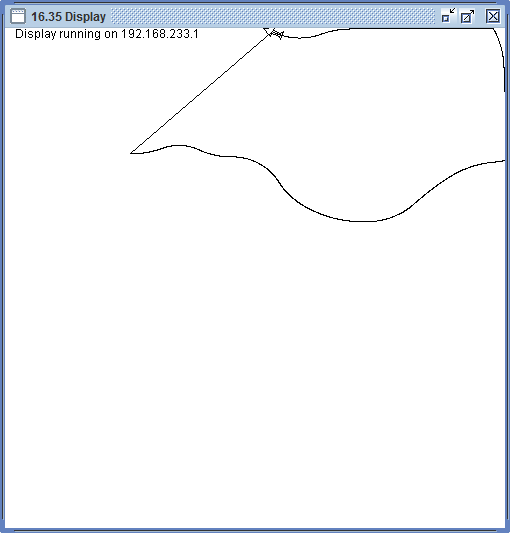
\includegraphics[width=0.7\linewidth]{random}
\caption{random}
\label{fig:random}
\end{figure}
\begin{figure}
\centering
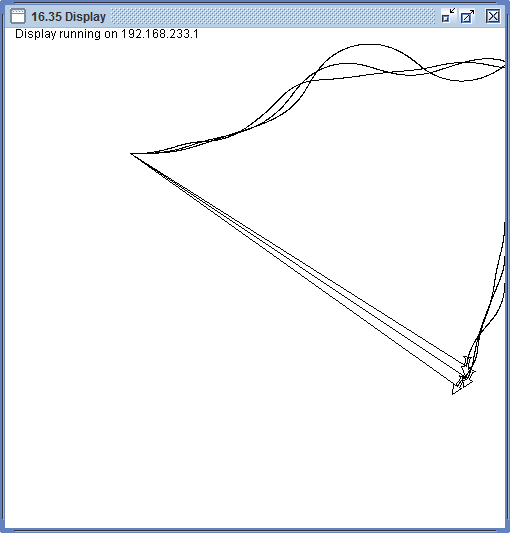
\includegraphics[width=0.7\linewidth]{follower}
\caption{follower}
\label{fig:follower}
\end{figure}



\end{document}